\begin{frame}{Relevant Questions}
    \textbf{RQ1: How can we evaluate the quality of a story?}
    \begin{itemize}
        \item What setting do we choose?
        \item Which criteria can be used to evaluate a story?
        \item What are the available automatic evaluation measures?
        \item How can we compare human and automatic evaluation methods?
    \end{itemize}
\end{frame}

\begin{frame}
    \frametitle{Definitions}
    \begin{definition}[{\asgfull} ({\asg})]
        Given a short sentence $p_i$ (called a \textbf{story-prompt}), the {\asg} task consists in using a language model that takes $p_i$ as its input for generating a story $y_i$.
    \end{definition}

    \begin{definition}[{\asefull} ({\ase})]
    Given an automatic evaluation measure $m$ ({\eg}\ a scoring algorithm, an \llm\dots), a story-prompt $p_i$, a candidate story $y_i$, and optional additional text $z_i$ ({\eg}\ a reference story), we define the {\ase} task as the production of an evaluation score $m(p_i, y_i, z_i)$, which we may write $m(y_i)$ for brevity.
    \end{definition}
\end{frame}

\begin{frame}{ASG Example}
    \begin{itemize}[<+->]
        \item \textbf{Story-prompt}: You swear that you keep seeing the same woman in blue every time you go on family vacation, when you turn 18, you are introduced to her.
        \item \textbf{Story generated by Platypus2-70B}: As a child, I always looked forward to going on family vacation. It was a time to unwind, enjoy nature, and most importantly, spend time with my loved ones. Yet, something strange always happened whenever we went on these trips. No matter where we went or what we did, I would inexplicably keep seeing the same woman in blue, almost as if she was following us. This mystery woman always wore a light blue summer dress and had her long dark hair styled into a loose braid. [...]
    \end{itemize}
    
\end{frame}

\begin{frame}{Human Criteria for Story Evaluation}
    \begin{itemize}[<+->]
        \item In the ASG literature, many criteria have been used:
        \item Coherence, Interestingness, Grammar, Sentence Preference, Faithfulness, Relevance / Fidelity, Fluency, Logicality, Overall Preference, Likability, Overall Quality, Outline Utilisation, Narrative Fow, Orering, Emotion Faithfulness, Content Quality, Human Plausibility, Ending Quality, Naturalness, etc.
        \item Many criteria \textbf{overlap} (Coherence / Logicality, Overall Quality / Content Quality...);
        \item Some of them are \textbf{not specific to ASG} (Grammar, Fluency...).
    \end{itemize}

\end{frame}

\begin{frame}{Human Criteria for Story Evaluation}
    We surveyed the {\asg} and social sciences literature to design the following set of evaluation criteria:
    \begin{enumerate}[<+(1)->]
        \item \textbf{Relevance} (\myre): ``how well the story matches its story-prompt'';
        \item \textbf{Coherence} (\mych): ``how much the story makes sense'';
        \item \textbf{Empathy} (\myem): ``how well the reader understood the character’s emotions'';
        \item \textbf{Surprise} (\mysu): ``how surprising the end of the story was'';
        \item \textbf{Engagement} (\myeg): ``how much the reader engaged with the story''; 
        \item \textbf{Complexity} (\mycx): ``how elaborate the story is''.
    \end{enumerate}
\end{frame}

\begin{frame}{Taxonomy of Evaluation Measures}
    We propose a bi-dimensional taxonomy of automatic measures:
    \uncover<2->{\begin{itemize}
        \item \textbf{Reference-based}: it compares a candidate story with a reference story written for the same prompt;
        \item \textbf{Reference-free}: it relies only on the candidate story (and, possibly, the prompt).
    \end{itemize}}
    \uncover<3->{and
    \begin{itemize}
        \item \textbf{String-based}: it evaluates the textual representation of the inputs;
        \item \textbf{Embedding-based}: it relies on word embeddings or contextualized embeddings;
        \item \textbf{Model-based}: it leverages regression or language models to return a score.
    \end{itemize}}
\end{frame}

\begin{frame}{Taxonomy of Evaluation Measures}
    \begin{table}[h]
        \scriptsize
        \centering
        \begin{tabular}{lcc}
        \toprule
          & \textbf{Reference-based} & \textbf{Reference-free} \\ 
        \midrule
        \multirow{6}{2.5cm}{\textbf{String-based}} & {\bleu} & \textsc{Coverage} \\
        & {\rouge} & \textsc{Density} \\
        & \textsc{METEOR} & \textsc{Compression} \\
        & \textsc{\textsc{chrF}} & \textsc{Text length} \\
        & \textsc{CIDEr} & \textsc{Novelty} \\
        & & \textsc{Repetition} \\
        \midrule
        \multirow{5}{2.5cm}{\textbf{Embedding-based}} & \textsc{ROUGE-WE} & \\
        & \textsc{BERTScore} & \\
        & \textsc{MoverScore} & \textsc{SUPERT} \\
        & \textsc{BaryScore} & \\
        & \textsc{DepthScore} \\
        \midrule
        \multirow{4}{2.5cm}{\textbf{Model-based}} & \textsc{S3} & \\
        & \textsc{SummaQA} & \textsc{BLANC} \\
        & \textsc{InfoLM} \\
        & \textsc{BARTScore} & \textsc{BARTScore} \\
        \bottomrule
        \end{tabular}
        \caption{Taxonomy of the automatic measures considered in our study.}
        \label{tab:measures}
    \end{table}
\end{frame}

\begin{frame}{Meta-Evaluation Framework}
    Objective: comparing evaluation methods between one another. Especially, we would like to ascertain \textbf{how well automatic measures correlate with human evaluation}, which we will use as our gold standard.
    \begin{block}{Notations}
        For $S$ systems and $N$ story-prompts, let $y_i^j$ be the story generated by system $j \in \{1,\dots,S\}$ for story-prompt $i \in \{1,\dots,N\}$.\\For a (human or automatic) measure $m$, we note $m(y_i^j)$ the score associated to $y_i^j$.
    \end{block}
\end{frame}

\begin{frame}{Kendall's Correlation Coefficient}
    We follow \citet{gilpin1993table, newson2002parameters} and choose to use Kendall's $\tau$ coefficient, a statistic used to measure the ordinal association between two measured quantities.
    \vspace*{-1em}
    \begin{figure}
        \centering
        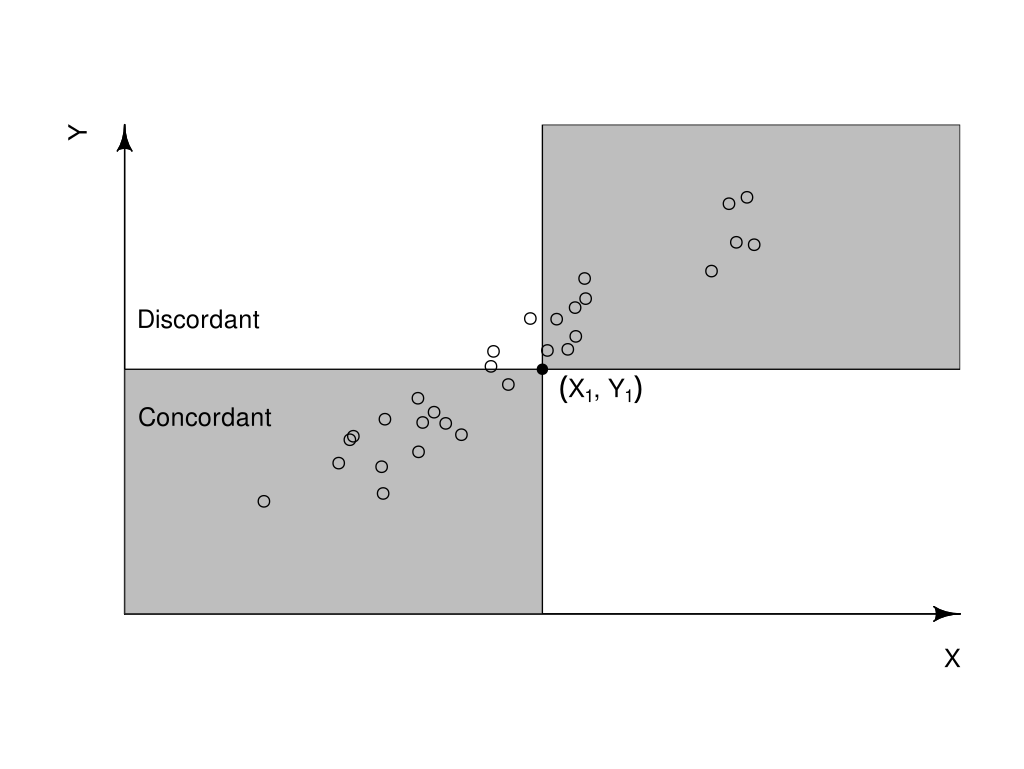
\includegraphics[width=0.5\linewidth]{pictures/kendall_correlation.png}
        \caption{Gray and white areas: respectively concordant and discordant points \wrt\ $(X_1,Y_1)$. 395 concordant pairs and 40 discordant pairs $\to$ $\tau = 0.816$.}
        \label{fig:kendall_correlation}
    \end{figure}
\end{frame}

\begin{frame}{Meta-Evaluation Strategies}
    \begin{definition}[System-level Correlation ($K^{\textrm{sys}}_{m_1,m_2}$)]
        This strategy measures \textbf{how suited $m_1$ is w.r.t.\ $m_2$ if used to compare the performance of two systems}. The correlation is applied to the mean values over all stories for all systems for both measures.
    \end{definition}
    \begin{definition}[Overall Correlation ($K^{\textrm{ovl}}_{m_1,m_2}$)]
        This strategy measures \textbf{how $m_1$ and $m_2$ agree at the level of the story itself}. It computes the correlation between the full vectors containing the scores of $m_1$ or $m_2$ for a given story for every system.
    \end{definition}
\end{frame}

\begin{frame}{Statistical Testing}
    \begin{itemize}
        \item To evaluate the statistical significance of observed increases in dependent correlations, we used the \textbf{Williams test} \citep{graham-baldwin-2014-testing}.
        \item To correct $p$-values for multiplicity, we used the \textbf{Benjamini-Hochberg procedure} \citep{benjamini1995controlling}.
    \end{itemize}
\end{frame}

\begin{frame}{Summary}
    \textbf{RQ1: How can we evaluate the quality of a story?}
    \begin{itemize}
        \item We defined our {\asg} and {\ase} settings;
        \item We designed 6 criteria for human evaluation: \textbf{Relevance}, \textbf{Coherence}, \textbf{Empathy}, \textbf{Surprise}, \textbf{Engagement}, and \textbf{Complexity};
        \item We proposed a taxonomy of automatic evaluation measures;
        \item We defined specific meta-evaluation strategies (system-level and overall correlations) and statistical testing procedures (Williams Test and Benjamini-Hochberg method).
    \end{itemize}
\end{frame}